\begin{frame}[fragile]
  \frametitle{Colecciones}

  \begin{enumerate}[1.]
    \item Listas    
  \end{enumerate}


  La lista es un tipo de colecci\'on ordenada, es equivalente  a lo que en otros lenguajes se conoce como arrays o vectores. Pueden contener cualquier tipo de dato: n\'umeros, cadenas,
booleanos, ... y tambi\'en listas.

  \begin{itemize}
    \item Ejemplo:
  \end{itemize}

  \begin{figure}
    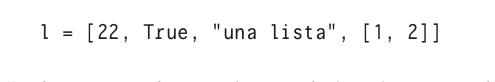
\includegraphics[width=0.6\textwidth]{Imagenes/Listas.jpg}
    \caption{\label{fig:Ejemplo1}Creaci\'on de una lista en Python.}
  \end{figure}  
 
 
\end{frame}

